\documentclass{article}
\usepackage[utf8]{inputenc}
\usepackage{listings}
\usepackage{parcolumns}
\usepackage{graphicx}
\usepackage[usenames,dvipsnames,svgnames,table]{xcolor}

\setlength\parindent{0pt}

\lstset{language=Java}
\definecolor{codegreen}{rgb}{0,0.6,0}
\definecolor{codegray}{rgb}{0.5,0.5,0.5}
\definecolor{codepurple}{rgb}{0.58,0,0.82}
\definecolor{backcolour}{rgb}{0.95,0.95,0.92}

\lstdefinestyle{mystyle}{
tabsize = 4,
showstringspaces = false,
numbers = left, 
commentstyle = \color{green},
keywordstyle = \color{blue}, 
stringstyle = \color{red}, 
rulecolor = \color{black}, 
basicstyle = \small \ttfamily ,
breaklines = true,
numberstyle = \tiny,
frame = shadowbox,
postbreak = \raisebox{0ex}[0ex][0ex]{\ensuremath{\hookrightarrow}}
}

\lstset{style=mystyle}

\title{Sistemi Operativi M}
\author{Federico Andrucci}
\date{September 2021}

\begin{document}

\maketitle
\tableofcontents
\cleardoublepage

\section{Virtualizzazione}

Virtualizzare un sistema (hardware e software) significa presentare all'uilizzatore una visione delle risorse del sistema diversa da quella reale.
Ciò è possibile introducendo un \textbf{livello di indirezione} tra la vista logica e quella fisica delle risorse.

Quindi l'obiettivo della virtualizzazione è quello di disaccoppiare il comportamento delle risorsedi un calcolatore dalla loro realizzazione fisica. 
Quindi apparendo diverse da quelle effettive della macchina. Il software che si occupa di virtualizzare in parole semplici divide le risorse reali nel numero di macchine virtuali necessarie. 
Quindi ogni macchina virtuale avrà la sua CPU, GPU, RAM, ecc...

Esmpi di virtualizzazione:
\begin{itemize}
    \item \textbf{Virtualizzazione a livello di processo:} i sistemi multitasking permettono l'esecuzione contemporanea di più processi, ognuno dei quale dispone 
    di una macchina virtuale dedicata. Questo tipo di virtualizzazione viene realizzata dal kernel del sistema operativo.
    \item \textbf{Virtualizzazione della memoria:} in presenza di memoria virtuale, ogni processo vede uno spazio di indirizzamento di dimensioni indipendenti dallo spazio fisico effettivamente a dispozione. Anche questa virtualizzaione è realizzata dal kernel.
    \item \textbf{Astrazione:} un oggetto astratto (risorsa virtuale) è la rappresentazione semplificata di un oggetto (risortsa fisica), quindi esibendo le 
    proprietà significative per l'utilizzatore e nascondendo i dettagli realizzativi non importanti
\end{itemize}

\subsection{Virtualizzazione di un Sistema di Elaborazione}
Tramite la virtualizzazione una singola piattaforma hardware viene condivisa da più elaboratori virtuali, ognuno gestito da un proprio sistema operativo.
Il disaccoppiamento viene realizzato dal \textbf{Virtual Machine Monitor (VMM)}, il cui compito è quello di consentire la condivisione da parte di più macchine 
virtuali di una singola piattaforma hardware.

Quindi il \textbf{VMM} è il \textbf{mediatore unico} nelle interazioni tra le macchine virtuali e
l'hardware, il quale garantisce: \textbf{isolamento tra le VM} e \textbf{stabilità del sistema}.

\subsection{Tecniche del VMM}
\subsubsection{Emulazione}
L'emulazione è l'insieme di tutti quei meccanismi che permettono l'esecuzione di un programma compilato su un determiato sistema di girare su un qualsiasi altro sistema differente da quello nel quale è stato compilato.
Quindi vengono emulate interamente le singole istruzioni dell'architettura ospitata.

I vantaggi dell'emulazione sono l'interoperabilità tra ambienti eterogenei, mentre gli svantaggi sono le ripercussioni sulle performances.

\vspace{5mm}
Esistono principalmente due tecniche di emulazione: \textbf{interpretazione} e \textbf{ricompilazione dimanica}.

\vspace{5mm}
\textbf{Interpretazione}:

L'interpretazione si basa sulla lettura di ogni singola istruzione del codice macchina che deve essere eseguito e sulla esecuzione di più istruzioni sull'host virtualizzante.
Produce un sovraccarico elevento in quanto potrebbero essere necessarie molte istruzioni dell'host per interpretare una singola istruzione sorgente.

\vspace{5mm}
\textbf{Compilazione dinamica}:

Invece di leggere una singola istruzione del sistema ospitato, legge interi blocchi di codice, vengono analizzati, tradotti per la nuova architettura, ottimizzati e messi in esecuzione.
Il vantaggio in termini prestazionali rispetto all'interpretazione è notevolmente maggiore.

Ad esempio parti di codice utilizzati frequentemente vengono bufferizzati nella cache per evitare di doverli ricompilare in seguito.


..
..
..


\subsection{Realizzaione del VMM}
\textbf{Requisiti di Popek e Goldberg del 1974}:

\begin{itemize}
    \item \textbf{Ambiente di esecuzione per i programmi sostanzialmente identico a quello della macchina reale}: Gli stessi programmi che eseguono nel sistema non virtualizzato possono essere eseguiti nelle VM
    senza modifiche e problemi.
    \item \textbf{Garantire un'elevata efficienza nell'esecuzione dei programmi}: Il VMM deve permettere l'esecuzione diretta delle istruzioni impartite dalle macchine virtuali, quindi le istruzioni non 
    privilegiate vengono eseguite direttamente in hardware senza coinvolgere il VMM
    \item \textbf{Garantire la stabilità e la sicurezza dell'intero sistema}: Il VMM deve sempre rimanere sempre nel pieno controllo delle risorse hardware, e i programmi in  esecuzione nelle macchine virtuali non possono 
    accedere all'hardware in modo privilegiato
\end{itemize}

\textbf{Parametri e classificazione}
\begin{itemize}
    \item \textbf{Livello} nel quale è collocato il VMM:
    \begin{itemize}
        \item \textbf{VMM di sistema}: eseguono direttamente sopra l'hardware del elaboratore (vmware, esx, xen, kvm)
        \item \textbf{VMM ospitati}: eseguiti come applicazioni sopra un S.O. esistente (parallels, virtualbox)
    \end{itemize}
    \item \textbf{Modalità di dialogo}: per l'accesso alle risorse fisiche tra le macchine virtuali ed il VMM:
    \begin{itemize}
        \item \textbf{Virtualizzazione pura} (vmware): le macchine virtuali usano la stessa interfaccia dell'architettura fisica
        \item \textbf{Paravirtualizzazione} (xen): il VMM presenta un'interfaccia diversa da quella dell'architettura HW
    \end{itemize}
\end{itemize}

\subsubsection{Ring di protezione}

La CPU prevede due livelli di protezione: \textbf{supervisore o kernel (0)} e \textbf{utente ($<$0)}.

Ogni ring corrisponde a una diversa modalità di funzionamento del processore:
\begin{itemize}
    \item a livello 0 vengono eseguite le istruzioni privilegiate della CPU
    \item nei ring di livello superiore a 0 le istruzioni privilegiate non vengono eseguite
\end{itemize}

Alcuni progrmmi sono progettati per eseguire nel ring 0, ad esempio il Kernel del S.O. infatti è l'unico componente che ha pieno controllo dell'hardware.

\vspace{3mm}
\textbf{VMM (vmm di sistema)}

In un sistema virtualizzato il VMM deve essere l'unica componente in grado di mantenere il controllo completo dell'hardware. Infatti solo il VMM opera nello stato supervisore, 
mentre il S.O. e le applicazioni eseguono in un ring di livello superiore.

Sorgono però due problemi:
\begin{itemize}
    \item \textbf{Ring deprivileging}: il s.o. della macchina virtuale esegue in un ring che non gli è proprio
    \item \textbf{Ring compression}: se i ring utilizzati sono solo 2, applicazioni e s.o. della macchina virtuale eseguono allo stesso livello: 
    scarsa protezione tra spazio del s.o. e delle applicazioni.
\end{itemize}

\subsubsection{Ring Deprivileging}
Con Ring Deprivilenging si indica una situazione nel quale l'esecuzione di istruzioni privilegiate richieste dal sistema operativo nell'ambiente guest non
possono essere eseguite in quanto richiederebbero un ring 0, ma il kernel della macchina virtuale esegue in un ring di livello superiore (foto telefono 1)

Una possibile prima soluzione è il \textbf{Trap \& Emulate}: nel quale se il guest tenta di eseguire un'istruzione privilegiata

\begin{itemize}
    \item la CPU notifica un'eccezione al VMM (\textbf{trap}) e gli trasferisce il controllo
    \item il VMM controlla la correttezza dell'operazione richiesta e ne emula il comportamento (\textbf{emulate})
\end{itemize}

Quindi in poche parole la CPU notifica e delega al VMM il controllo e l'esecuzione dell'istruzione privilegiata.

Esempio:

Il guest tenta di disabilitare le interruzioni (popf), se la richiesta della macchina virtuale fosse eseguita direttamente sulla CPU sarebbero disabilitati
tutti gli interrupt di sistema e quindi il VMM non potrebbe riottenere il controllo. Invece, con Trap\&Emulate riceve la notifica di tale richiesta e ne emula
il comportamento sospendendo gli interrupt solamente per la macchina virtuale richiedente.

\vspace{3mm}
\textbf{Supporto HW alla virtualizzazione}

L'archietettura della CPU si dice \textbf{naturalmente virtualizzabile} se e solo se prevede l'invio di trap al VMM per ogni istruzione privilegiata invocata da un
livello di protezione differente dal quello del VMM.

Se la CPU è naturalmente virtualizzabile viene implementato il trap\&emulate, altrimenti, se non è virtualizzabile vi sono 2 possibilità: \textbf{Fast Binary Translation} e 
\textbf{Paravirtualizzazione}.

\subsubsection{Fast Binary Translation}
Il VMM scansiona dinamicamente il codice dei sistemi operativi guest prima dell'esecuzione per sostituire a run time i blocchi contenenti istuzioni privilegiate
in blocchi equivalenti dal punto di vista funzionale e contenenti chiamate al VMM. Inoltre i blocchi tradotti sono eseguiti e conservati in cache per eventuali
riusi futuri. (SISTEMARE)

(immagine slide 33)

Il principale limite della Fast Binary Translation è che la traduzione dinamica è molto costosa. Però, con questa tecnica, ogni macchina virtuale è una esatta
copia della macchina fisica, con la possiblità di installare gli stessi s.o. di architetture non virtualizzate.

\subsubsection{Paravirtualizzazione}
Il VMM (hypervison) offre al sistema operativo guest un'interfaccia virtuale (ovviamente differente da quello hardware del processore) chiamata **hypercall API**
alla quale i s.o. guest devono rifersi per avere accesso alle risorse (system call).

Queste Hypercall API permettono di:
\begin{itemize}
    \item richiedere l'esecuzione di istruzioni privilegiate, senza generare un interrupt al VMM
    \item i kernel dei s.o. guest devono quindi essere modificati per avere accesso all'interfaccia del particolare VMM
    \item la struttura del VMM è semplificata perchè non deve più preoccuparsi di tradurre dinamicamente i tentativi di operazioni privilegiate dei s.o. guest
\end{itemize}

Le prestazioni rispetto alla Fast Binary Translation sono notevolmente superiori, però ovviamente c'è una necessità di porting dei dei s.o. guest (non sempre facile).

(aggiungere protezione processore)


\section{La protezione nei Sistemi Operativi}

\textbf{Sicurezza}: riguarda l'insieme delle tecniche per regolamentare l'accesso degli utenti al sistema di elaborazione. La sicurezza impedisce accessi
non autorizzati al sistema e i conseguenti tentativi dolosi di alterazione e distruzione di dati.

\vspace{3mm}
\textbf{Protezione}: insieme di attività volte a garantire il controllo dell'accesso alle risorse logiche e fisiche da parte degli utenti autorizzati
all'uso di un sistema di calcolo.

La sicurezza mette a disposizione meccanismi di **identificazione, autenticazione, ...**

Per rendere un sistema sicuro è necessario stabilire per ogni utente autorizzato:
\begin{itemize}
    \item quali siano le risore alle quali può accedere
    \item con quali operazioni può accedervi
\end{itemize}

Tutto ciò è stabilito dal sistema di protezione attraverso delle tecniche di controllo dell'accesso.

In un sistema il controllo degli accessi si esprime tramite la definizione di tre livelli concettuali:
\begin{itemize}
    \item modelli
    \item politiche
    \item meccanismi
\end{itemize}

\vspace{3mm}
\textbf{Modelli:}

Un modello di protezione definisce i soggetti, gli oggetti e i diritti d'accesso:
\begin{itemize}
    \item \textbf{oggetti}: costituiscono la parte passiva, cioè le risorse fisiche e logiche alle quali si può accedere e su cui si può operare.
    \item \textbf{soggetti}: rappresentano la parte attiva di un sistema, cioè le eintità che possono richiedere l'accesso alle risorse (utenti e processi)
    \item \textbf{diritti d'accesso}: sono le operazioni con le quali è possibile operare sugli oggetti
\end{itemize}

(Un soggetto può avere diritti d'accesso sia per gli oggetti che per gli altri soggetti)

Ad ogni soggetto è associato un \textbf{dominio di protezione}, che rappresenta l'ambiente di protezione nel quale il soggetto esegue. Quindi il dominio
indica i diritti d'accesso posseduti dal sogetto nei confronti di ogni risorsa.

Un dominio di protezioen è unico per ogni soggetto, mentre un processo può eventualmente cambiare dominio durante la sua esecuzione.

\vspace{3mm}
\textbf{Politiche:}

Le \textbf{politiche di protezione} definiscono le regole con le quali i soggetti possono accedere agli oggetti
Classificazione delle politiche:
\begin{itemize}
    \item \textbf{discretional access control (DAC)}: il creatore di un oggetto controlla i diritti di accesso per quell'oggetto (unix). La definizione delle politiche è
    decentralizzata.
    \item \textbf{mandatory access control (MAC)}: i diritti di accesso vengono definiti in modo centralizzato. Ad esempio in installazioni di alta sicurezza
    \item \textbf{role based access control (RBAC)}: ad un ruolo sono assegnati specifici diritti di accesso sulle risorse. Sli utenti possono appartenere a diversi
    ruoli. I diritti attribuiti ad ogni ruolo vengono assegnati in modo centralizzato
\end{itemize}

\vspace{3mm}
\textbf{Principio del privilegio minimo}: ad ogni soggetto sono garantiti i diritti d'accesso solo agli oggetti strettamente necessari per la sua esecuzione
(POLA: principle of least authority). il POLA è una caratteristicha desiderabile in ogni sistema di controllo.
\vspace{3mm}

\textbf{Meccanismi:}

I \textbf{meccanismi di protezione} sono gli strumenti necessari a mettere in atto una determinata politica.
Principi di realizzazione:
\begin{itemize}
    \item \textbf{Flessibilità del sistema di protezione}: i meccanismi devono essere sufficientemente generali per consentire l'applicazione di diverse politiche 
    di protezione
    \item \textbf{Separazione tra meccanismi e politiche}: la politicha definische "cosa va fatto" ed il meccanismo "come va fatto". Ovviamente è desiderata la
    massima indipendenza tra le due componenti.
\end{itemize}

\subsection{Dominio di protezione}
Un dominio definisce un insiem edi coppie, ognuna contenente l'identificatore di un oggetto e l'insieme delle operazioni che il soggetto associato al
dominio può eseguire su ciascun oggetto

\vspace{3mm}
$D(S)$ = $\{$$<$o, diritti$>$ $|$ o è un oggetto, diritti è un insieme di operazioni$\}$
\vspace{3mm}

\textbf{Modello di Grahmm-Denning}

Questo modello forsnisce una serie di comandi che garantiscono la modifica controllata dello stato di protezione:
\begin{itemize}
    \item create object
    \item delete object
    \item create subject
    \item delete subject
    \item read access right
    \item grant access right
    \item delete access right
    \item tranfer access right
\end{itemize}

\vspace{3mm}
\subsubsection{Diritti}

\textbf{Diritto Owner}:
\vspace{3mm}

Il diritto owner permette l'assegnazioen di qualunque diritto di accesso su un oggetto X ad un qualunque soggetto Sj da parte di un soggetto Si. L'operazione è consentita solo
se il diritto owner appartiene a A[Si, X]

\vspace{3mm}
\textbf{Diritto Control}:
\vspace{3mm}

Eliminazione di un diritto di accesso per un oggetto X nel dominio di Sj da parte di Si. L'operazione è consentita solo se il diritto control appartiene a A[Si, Sj], oppure owner
appartiene a A[Si, X].

\vspace{3mm}
\textbf{Cambio di dominio: switch}
\vspace{3mm}

Il cambio di dominio permette che un processo che esegue nel dominio del soggetto si può commutare al dominio di un altro soggetto Sj.
L'operazione è consentita solo se il diritto switch appartiene a A[Si, Sj].

\subsection{Realizzazione della matrice delgi accessi}
La matrice degli accessi è una notazione astratta che rappresenta lo stato di protezione. Nella rappresentazione concreta è necessario considerare: la dimensione della matrice e matrice 
sparsa.

La rappresentazione concreta della matrice degli accessi deve essere ottimizzata sia riguardo all'occupazione di memoria sia rispetto all'efficienza nell'accesso e nella gestione della
informazioni di protezione.
Ci sono principalmente di approcci:
\begin{itemize}
    \item \textbf{Access Control List (ACL)}: rappresentazione per colonne, per ogni oggetto è associata una lista che contiene tutti i soggetti che possono accedere all'oggetto, con i relativi diritti
    d'accesso per l'oggetto
    \item \textbf{Capability List}: rappresentazione per righe, ad ognin soggetto è associata una lista che contiene gli oggetti accessibili dal soggetto ed i relativi diritti d'accesso.
\end{itemize}

\subsubsection{Access Control List}
La lista degli accessi per ogni oggetto è rappresentata dall'insieme delle coppie: \textbf{$<$soggetto, insieme dei diritti$>$}
limitatamente ai soggetti con un insieme non vuoto di diritti per l'oggetto.

Quando deve essere eseguita un'operazione M su un oggetto Oj, da parte di Si, si cerca nella lista degli accessi \textbf{$<$Si, Rk$>$, con M appartenente a Rk}.

La ricerca può essere fatta preventivamente in una lista di default contenete i diritti di accesso applicabili a tutti gli oggetti. 
Se in entrambi i casi la risposta è negativa, l'accesso è negato.

\vspace{3mm}
\textbf{Utenti e Gruppi}
\vspace{3mm}

Generalmente ogni soggetto rappresenta un singolo utente. Molti sistemi hanno il concetto di \textbf{gruppo di utenti}. I gruppi hanno un nome e possono essere inclusi nella ACL.

In questo caso l'entry in ACL ha la forma:
\textbf{UID-1, GID-1 : $<$insieme di diritti$>$}

\textbf{UID-2, GID-2 : $<$insieme di diritti$>$}

Dove UID è lo user identifier e GID è il group identifier.

\vspace{3mm}
In certi casi il gruppo identifica un ruolo: uno stesso utente può appartenere a gruppi diversi e quindi  con diritti diversi. In questo caso, quando un utente accede, specifica il
gruppo di appartenenza.

\subsubsection{Capability List}
La lista delle capability, per ogni soggetto, è la lista di elementi ognuno dei quali:
\begin{itemize}
    \item è associato a un oggetto a cui il soggetto può accedere
    \item contiene i diritti di accessi consentiti su tale oggetto
\end{itemize}

\vspace{3mm}
Ogni elemento della lista prende il nome di \textbf{capability}. Il quale di compone di un identificatore (o un indirizzo) che indica l'oggetto e la rappresentazione dei vari diritti d'accesso.
Quando S intende eseguire un'operazione M su un oggetto Oj: il meccanismo di protezione controlla se nella lisra delle capability associata a S ne esiste una relativa ad Oj che abbia
tra i suoi diritti M.

\vspace{3mm}
Ovviamente le Capability List devono essere protette da manomissioni, ed è possibile in diversi modi:
\begin{itemize}
    \item la capability list viene gestita solamente da s.o.; l'utente fa riferimento ad un puntatore (capability) che identifica la sua posizione nella lista appartenete allo spazio del kerner
    \item Architettura etichettata: a livello HW, ogni singola parola ha bit extra, che esprimono la protezione su quella cella di memoria. Ad esempio, se è una capability, deve essere
    protetta da scritture non autorizzate.
\end{itemize}

\vspace{3mm}
I bit tag non sono utilizzari dall'aritmetica, dai confronti e da altre istruzioni normali e può essere modificato solo da programmi che agiscono in modo kernel.

\vspace{3mm}
\subsubsection{Revoca dei diritti di accesso}

In un sistema di protezione dinamica può essere necessario revocare i diritti d'accesso per un oggetto. La revoca può essere di tre tipi:
\begin{itemize}
    \item \textbf{generale o selettiva}: cioè valere per tutti gli utenti che hanno quel diritto di accesso o solo per un gruppo
    \item \textbf{parziale o totale}: cipè riguardare un sottoinsieme di diritti per l'oggetto, o tutti
    \item \textbf{temporanea o permanente}: cioè il diritto di accesso non sarà più disponibile, oppure potrà essere successivamente riottenuto
\end{itemize}

\vspace{3mm}
\textbf{Revoca del diritto per un oggetto con ACL}:

Si fa riferimento alla ACL associata all'oggetto e si cancellano i diritti di accesso che si vogliono revocare

\vspace{3mm}
\textbf{Revoca del diritto per un oggetto con Capability List}:

Più complicato rispetto ad ACL. È necessario verificare per ogni dominio se contiene la capability con riferimento all'oggetto considerato.

\subsection{Protezione e Sicurezza}

La protezione riguarda solamente il controllo degli accessi alle risorse interne al sistema. Invece la sicurezza si occupa di controllare gli accessi al sistema stesso.

In alcuni casi la sola protezione può non essere efficace, nel caso in cui, ad esempio, un utente autorizzato riesce a far eseguire programmi che agiscono sulle
risorse del sistema.

\subsubsection{Sicurezza Multilivello}

La maggior parte dei sistemi operativi permette ai singoli utenti di determinare chi possa leggere e scrivere i loro file ed oggetti. Invece in acluni ambienti
è richiesto e necessario un più stretto controllo sulle regole di accesso alle risorse (ambiente militare, ospedaliero, ecc). Vengono quindi stabilite delle regole
\textbf{generali} su "chi può accedere e a che cosa", che possono essere modificate solo da un'entità centrale autorizzata.

Quando è necessario un controllo obbligatorio degli accessi al sistema, l'organizzazione a cui il sistema appartiene definisce le politiche \textbf{MAC} che
stabiliscono le \textbf{regole generali} tramite l'adozione di un modello di sicurezza.

\vspace{3mm}
I modelli di sicurezza più utilizzati sono:
\begin{itemize}
    \item modello \textbf{Bell-La Padula}
    \item modello \textbf{Biba}
\end{itemize}

Entrambi sono modelli multilivello.

\vspace{3mm}
In un modello di sicurezza multilivello i \textbf{soggetti} (utenti) e gli \textbf{oggetti} (risorse, file, ecc) sono \textbf{classificati} in \textbf{livelli} (classi
di accesso):
\begin{itemize}
    \item Livelli per i soggetti (\textbf{clearance levels})
    \item Livelli per gli oggetti (\textbf{sensivity levels})
\end{itemize}

\vspace{3mm}
Il modello inoltre fissa le \textbf{regole di sicurezza}, le quali controllano il flusso delle informazioni tra i livelli.

\vspace{3mm}
\textbf{Modello Bell-La Padula}
\vspace{3mm}

Modello progettato per realizzare la sicurezza in organizzazioni militari, garantendo la \textbf{confidenzialità} delle informazioni.

Associa a un sistema di protezione (matrice degli accesso) due regole di sicurezza MAC, che stabiliscono la direzione di propagazione delle informazioni nel sistema.

\vspace{3mm}
Quattro livelli di sensibilità degli oggetti:
\begin{itemize}
    \item Non classificato
    \item Confidenziale
    \item Segreto
    \item Top secret
\end{itemize}

\vspace{3mm}
Quattro livelli di autorizzazione (clearance) per i soggetti:

Le persone sono assegnate ai livelli a seconda del ruolo nell'organizzazione.

\vspace{3mm}
\textbf{Regole di Sicurezza}:
\begin{itemize}
    \item \textbf{Proprietà di semplice sicurezza}: un processo in esecuzione al livello di sicurezza k può leggere solo oggetti al suo livello o a livelli inferiori
    \item \textbf{Proprietà *}: un processo in esecuzione al livello di sicurezza k può scrivere solamente oggetti al suo livello o a quelli superiori
\end{itemize}

Quindi i processi possono leggere verso il basso e scrivere verso l'alto, ma non il contrario. (flusso delle informazioni dal basso verso l'alto).

\vspace{3mm}
Generalmente a queste regole si aggiungono le regole di protezioen speficicate dalla matrice degli accessi.

\begin{figure}[htbp]
    \centering
    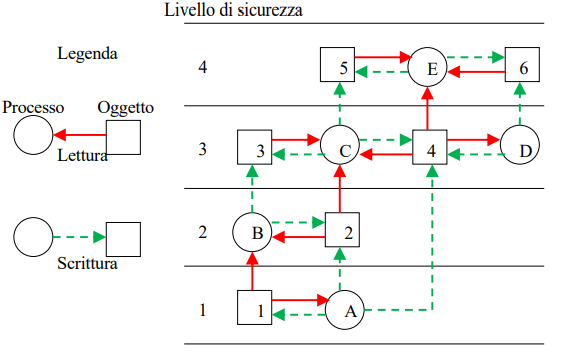
\includegraphics[width=0.70\columnwidth]{imgs/bell-padula.PNG}
\end{figure}

\vspace{3mm}
Il modello Bell-La Padula è stato concepito per mantenere i segreti, non per garantire l'integrità dei dati. E\' possibile infatti sovrascrivere l'informazione
appartenente ad un livello superiore.

\vspace{3mm}
Esempio cavallo di troia

\vspace{3mm}
\textbf{Modello Biba}
\vspace{3mm}

Se il modello Bell-La Padula è stato concepito per mantenere i segreti e non per garantire l'integrità dei dati, il Modello Biba ha come obiettivo principale proprio
l'integrità dei dati.

\vspace{3mm}
\begin{itemize}
    \item \textbf{Proprietà di semplice sicurezza:} un processo in esecuzione al livello di sicurezza k può scrivere solamente oggetti al suo livello o a quelli
    inferiori (nessuna scrittua verso l'alto)
    \item \textbf{Proprietò di integrità *}: un processo in esecuzione al livello k può leggere solo oggetti al suo livello o quelli superiori (nessuna lettura
    verso il basso)
\end{itemize}

Ovviamente il modello Biba è in conflitto con il modello B-LP e quindi non possono essere utilizzati contemporaneamente.

\subsubsection{Architettura dei sistemi ad elevata sicurezza}

\textbf{Sistemi operativi sicuri, o fidati}: sistemi per i quali è possibile definire formalmente dei requisiti di sicurezza.

\vspace{3mm}
\textbf{Reference Monitor}: è un elemento di controllo realizzato dall'hardware e dal S.O. che regola l'accesso dei soggetti agli oggetti sulla base di paramentri
di sicurezza (es. modello Bell-La Padula)

\vspace{3mm}
\textbf{Trusted computing base}: il RM ha accesso ad una base di calcolo fidata (Trusted computing base, o TBC) che contiene:
\begin{itemize}
    \item Privilegi dei sicurezza (autorizzazioni di sicurezza) di ogni soggetto
    \item Attributi (classificazione rispetto alla sicurezza) di ciascun oggetto
\end{itemize}

\begin{figure}[htbp]
    \centering
    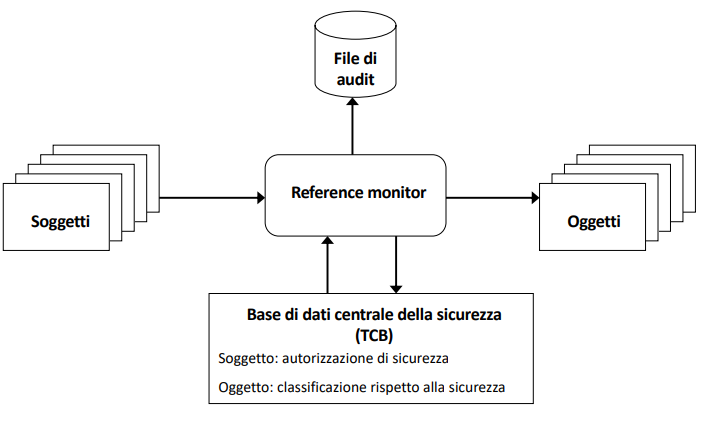
\includegraphics[width=0.70\columnwidth]{imgs/elevata_sicurezza.PNG}
\end{figure}

\vspace{3mm}
\textbf{Sistemi fidati}
\vspace{3mm}

Il RM impone le regole di sicurezza (B-LP: no read-up, no write-down) ed ha le seguenti proprietà:
\begin{itemize}
    \item \textbf{Mediazione completa}: le regole di sicurezza vengono applicate ad ogni accesso e non solo, ad esempio, quando viene aperto un file
    \item \textbf{Isolamento}: il monitor dei riferimenti e la base di dati sono protetti rispetto a modifiche non autorizzate (es. kernel)
    \item \textbf{Verificabilità}: la correttezza del RM deve essere provata, cioè deve essere possibile dimostrare formalmente che il monitor impone le regole
    di sicurezza e fornisce mediazione completa ed isolamento
\end{itemize}

\vspace{3mm}
Il requisito di \textbf{mediazione completa} rende preferibile, per motivi di efficienza, che la soluzione debba essere almeno parziamente hardware.

\vspace{3mm}
Il requisito di \textbf{isolamento} impone che non sia possibile oer chi porta l'attacco, modificare la logica del RM o il contenuto del DB centrale della sicurezza.

\vspace{3mm}
Il requisito della \textbf{verificabilità} è difficile da soddisfare per un sistema general-purpose.

\section{Programmazione Concorrente}


\section{Modello a memoria comune}

Esistono 2 principali modelli di interazione tra i processi:
\begin{itemize}
    \item Modello a \textbf{memoria comune} (ambiente globale, shared memory)
    \item Modello a \textbf{scambio di messaggi} (ambiente locale, distributed memory)
\end{itemize}

Il modello a memoria comune rappresenta la più semplice astrazione del funzionamento di un sistema in multiprogrammazione costituito da uno o più processi che hanno accesso
ad una memoria comune.

Ogni appliczione viene strutturata come un insieme di componenti, suddiviso in due sottoinsieme disgiunti:
\begin{itemize}
    \item \textbf{Processi} (componenti attivi)
    \item \textbf{Risorse} (componenti passivi)
\end{itemize}

Le Risorse rappresentatno un qualunque oggettim fisico o logico, di cui un processo necessita per portare a termine il suo compito.
Le risorse vengono raggruppate in classi, dove una classe rappresenta l'insieme di tutte e sole le operazioni che un processo può eseguire per operare su risorse di quella classe,

Ovviamente ci deve essere la necessità di specificare quali processi ed in quali istanti possono accedere alla risorsa. Quindi il \textbf{meccanismo di controllo degli accessi}
si occupa di controllare che gli accessi dei processi alle risorse avvengano correttamente.

\subsection{Gestore delle Risorse}

Per ogni risorsa \textbf{R}, il suo gestore definisce, in ogni istante t, \textbf{l'insieme SR(t) dei processi che, in tale istante, hanno il diritto di operare su R}.

\vspace{5mm}

Classificazione delle risorse:
\begin{itemize}
    \item Risorsa R \textbf{dedicata}: se SR(t) ha una caardianlità sempre <= 1
    \item Risorsa R \textbf{condivisa}: in caso contrario
    \item Risorsa R \textbf{allocata staticamente}: se SR(t) è una costante, quindi se SR(t) = SR(t0) per ogni t
    \item Risorsa R \textbf{allocata dinamicamente}: se SR(t) è funzione del tempo
\end{itemize}

\begin{figure}[htbp]
    \centering
    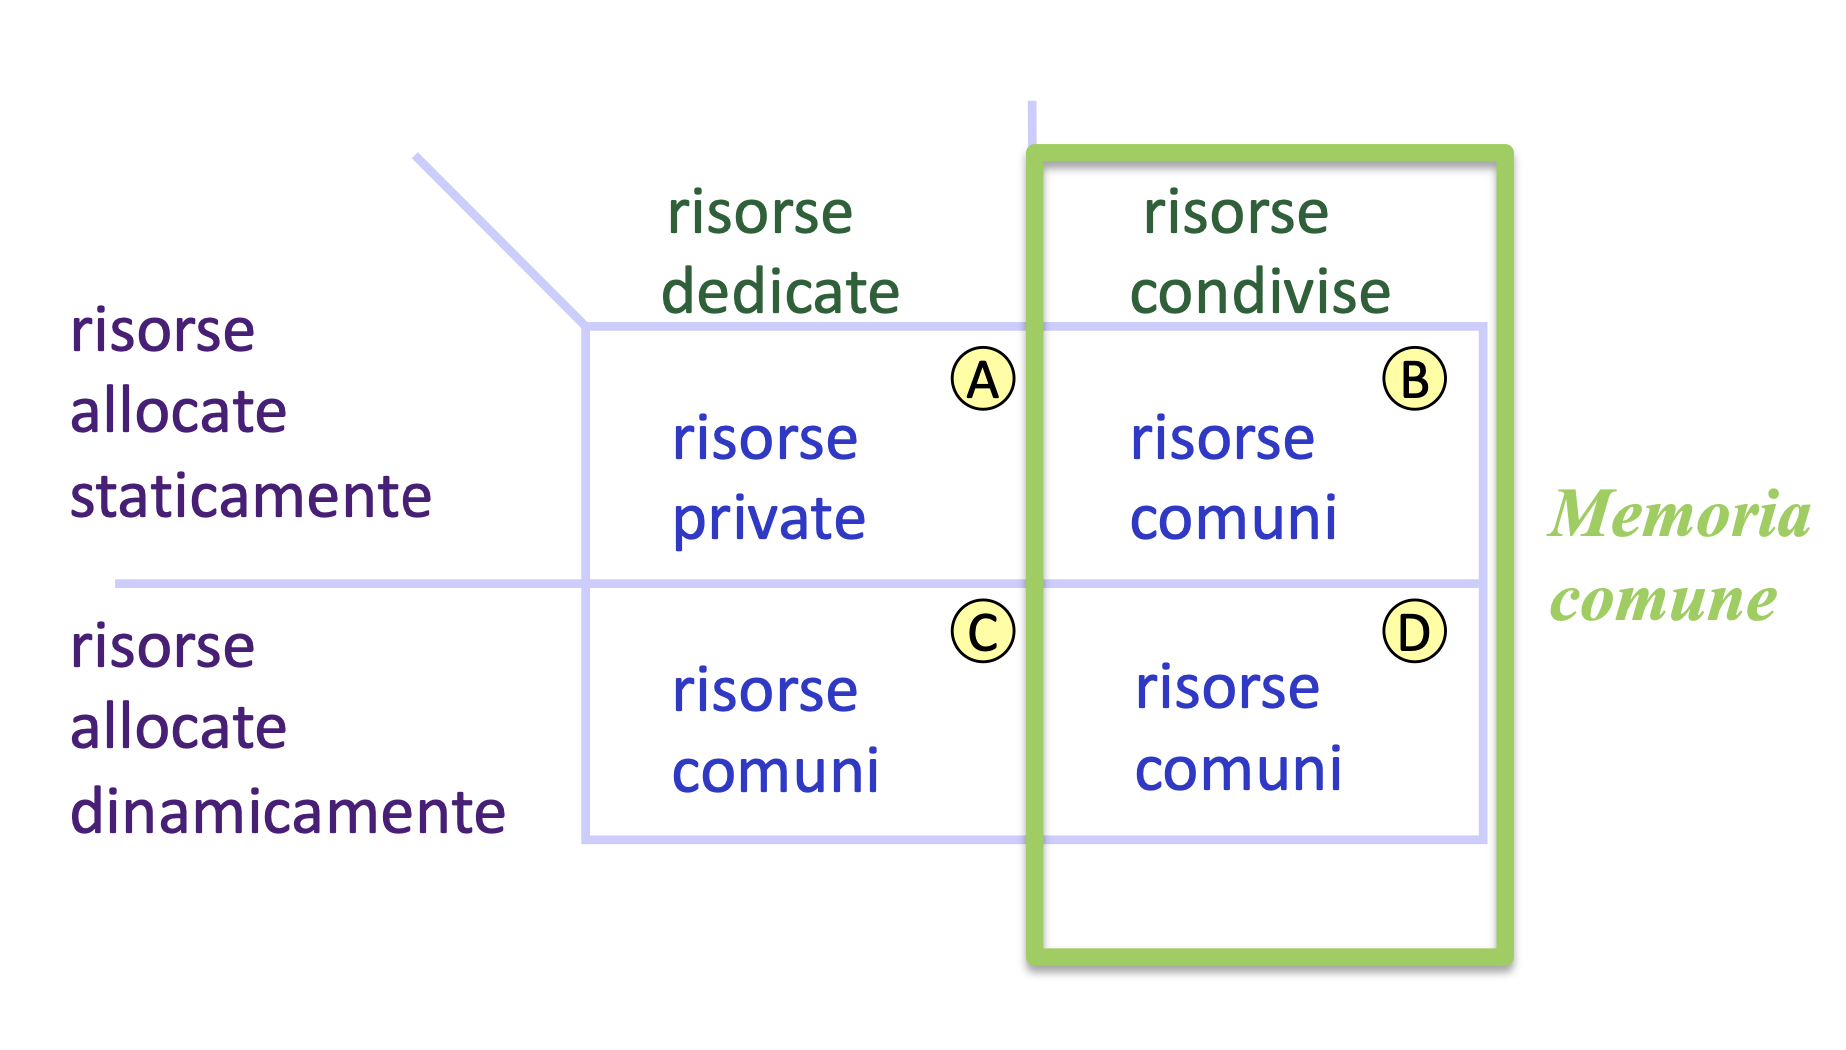
\includegraphics[width=0.50\columnwidth]{imgs/tipologie_allocazione.png}
\end{figure}

Per ogni risorsa \textbf{allocata staticamente}, l'insieme SR(t) è definito prima che il programma inizi la propria esecuzione; il gestore della risorsa è il programmatore che,
in base alle regole del linguaggio, stabilisce quale processo può vedere e quindi operare su R.


Per ogni risorsa \textbf{allocata dinamicamente}, il relativo gestore GR definisce l'insieme SR(t) in fase di esecuzione e quindi deve essere un componente della stessa applicazione,
nel quale l'allocazione viene decisa a run-time in base a politiche date.

\vspace{5mm}
Quindi i principali compiti del Gestore delle risorse sono:
\begin{itemize}
    \item mantenere \textbf{aggiornato} l'insieme SR(t) e cioè lo stato di allocazione della risorsa
    \item fornire i \textbf{meccanismi} che un processo può utilizzare per acquisire il diritto di operare sulla risorsa, entrando a far parte dell'insieme SR(t), e per rilasciare
    tale diritto quando non è più necessario
    \item implementare la \textbf{startegia} di allocazione della risorsa e cioè definire quando, a chi e per quanto tempo allocare la risorsa.
\end{itemize}

\vspace{5mm}
{\large \textbf{Accesso a Risorse}}
Consideriamo un processo P che deve operare, ad un certo istante, su una risorsa R di tipo T:

Se R è allocata \textbf{staticamente} a P (modalità A e B), il processo, se appartiene a SR, possiede diritto di operare su R in qualunque istante.
\vspace{3mm}
\begin{lstlisting}
R.op(...);
\end{lstlisting}

Se R è allocata \textbf{dinamicamente} a P (modalità C e D), è necessario prevedere un gestore GR, che implementa le funzioni di Richiesta e Rilascio della risorsa; quindi il
processo P deve seguire il seguente protocollo:

\vspace{3mm}
\begin{lstlisting}
GR.Richiesta(...);  // acquisizione della risorsa
R.op(...);          // esecuzione dell'operazione op su R
GR.Rilascio(...);   // rilascio della risorsa R
\end{lstlisting}

\vspace{3mm}
Se R è allocata come \textbf{risorsa condivisa}, (modalità B e D) è necessario assicurare che gli accessi avvengano in modo non divisibile: nel senso che òe funzioni di accesso alla
risorsa devono essere programmate come una \textbf{classe di sezioni critiche}, utilizzando meccanismi di sincronizzazione offerti dal linguaggio di programmazione e supportati
dalla macchina concorrente.

\vspace{3mm}
Se R è allocata come \textbf{risorsa dedicata}, (modalità A e C), essendo P l'unico processo che accede alla risorsa, non è necessario prevedere alcuna forma di sincronizzazione.

\vspace{5mm}
{\large \textbf{Regione critica condizionale [Hoare, Brinch-hansen]}}
Formalismo che permette di esprimere la specifica di qualunque vincolo di sincronizzazione. Data una risorsa R condivisa:

\begin{lstlisting}
region R << Sa; when(C) Sb; >>
\end{lstlisting}

\begin{itemize}
    \item tra doppie parentesi angolai il \textbf{corpo} della region che rappresenta una operazione da eseguire su una risorsa condivisa R e quindi costituisce una sezione critica
    che deve essere eseguita in \textbf{mutua esclusione} con le altre operazioni definite su R
    \item il corpo della region è costituito da due istruzioni da eseguire in sequenza: l'istruzione \textbf{Sa} e successivamente l'istruzione \textbf{Sb}
    \item in particolare, una volta terminata l'esecizione di Sa viene valutata la condizione \textbf{C}:
    \begin{itemize}
        \item se C è \textbf{vera} l'esecuzione continua con Sb
        \item se C + \textbf{false} il processo che ha invocato l'operazione attende che la condizione C diventi vera. Non appena C sarà vera l'esecuzione della region potrà riprendere
        ed eseguire Sb
    \end{itemize}
\end{itemize}

Esistono però dei casi particolari di regioni critiche:
\begin{itemize}
    \item \textbf{region R $<<$ S; $>>$}: specifica della sola mutua esclusione, senza ulteriori vincoli
    \item \textbf{region R $<<$ when(C) $>>$}: specifica di un semplice vincolo di sincronizzazione, nel quale il processo deve attendere che C sia verificata prima di proseguire
    \item \textbf{region R $<<$ when(C) S; $>>$}: specifica il caso dìin cui la condizione C di sincronizzazione caratterizza lo stato in cui la risorsa R deve trovarsi per poter
    eseguire l'operazione S (C quindi è una precondizione di S)
\end{itemize}

\subsection{Mutua Esclusione}

Il probelma della mutua esclusione nasce quando più di un processo alla volta può e deve accedere a variabili comuni. Quindi è di fondamentale importanza che le operazioni con le quali
i processi accedono alle variabili comuni non si sovrappongano nel tempo.

\vspace{3mm}
Con sezione critica s'intende la sequenza di istruzioni con le quali un processo accede e modifica un insieme di variabili comuni. Ad un insieme di variabili comuni possono
essere associate una sola sezione critica (usata da tutti i processi) oppure più sezioni critiche (classe di sezioni critiche).

La regola della mutua esclusione stabilisce che:
\begin{center}
    \textbf{Sezioni critiche appartenenti alla atessa classe devono escludersi mutuamente nel tempo.}
    \vspace{3mm}

    oppure

    \vspace{3mm}
    \textbf{Ad ogni istante può essere "in esecuzione" al più una sezione critica di ogni classe.}
\end{center}

\vspace{3mm}
Per specificare una sezione critica \textbf{S} che opera su una risorsa condivisa R:

\begin{lstlisting}
    <prologo>
        S;
    <epilogo>
\end{lstlisting}

Attraverso il \textbf{prologo} si ottiene l'autorizzazione ad eseguire la sezione critica, quindi R viene acquisita in modo esclusivo. Invece attraverso l'\textbf{epilogo}
la risorsa R viene liberata.

\vspace{5mm}
Le principali soluzioni possibili alla mutua esclusine sono:
\begin{itemize}
    \item \textbf{Algoritmiche:} (es. Algoritmi di Dekker, ecc.) la soluzione non necessita di meccanismi di sincronizzazione (es. semafori, lock, ecc.), ma sfrutta
    solo la possibilità di condivisione di variabili; l'attesa di un processo che trova la variabile condivisa già occupata viene modellata attraverso cicli di attesa attiva
    \item \textbf{Hardware-based:} ad esempio disabilitazione delle interruzioni, lock/unlock. Quindi il supporto è fornito direttamente dall'architettura HW.
    \item \textbf{Strumenti software di sincronizzazione realizzati dal nucleo della macchina concorrente:} prologo ed epilogo sfruttano strumenti di sincronizzazione
    che consentono l'effettiva sospensione dei processi in attesa ed eseguire sezioni critiche.
\end{itemize}

\subsection{Strumenti linguistici per la programmazione di interazioni}
\subsubsection{Il Semaforo}

Il semaforo è uno strumento linguistico di basso livello che consente di risolvere qualunque problema di sincronizzazione nel modello a memoria comune.

E\' realizzato dal nucleo della macchina concorrente. L'eventuale attesa nella esecuzione può essere realizzata utilizzando i meccanismi di gestione dei thread offerti
dal nucleo. Inoltre viene utilizzato per realizzaer strumenti di sincronizzazione di puù alto livello ad esempio le \textit{condition}.

\vspace{3mm}
\textbf{Definizione:} un semaforo è una \textbf{variabile intera non negativa}, alla quale è possibile accedere solo \textbf{tramite le due operazioni P e V}.
\vspace{3mm}

Definizione di un oggetto di tipo \textbf{semaphore}:
\begin{lstlisting}
    semaphore s = i;    // dove i (i >= 0) è il valore iniziale
\end{lstlisting}

Al tipo semaphore sono associati:
\begin{center}
    Insieme di valori = $\{X | X \in N\}$
    \vspace{3mm}

    Insieme delle operazioni = $\{P, V\}$
\end{center}

\vspace{5mm}
\textbf{Operazioni sul semaforo}
\vspace{3mm}

Un oggetto di tipo semaphore è condivisibile da due o più threads, che operano su di esso attraverso le operazioni \textbf{P} e \textbf{V}.

\begin{lstlisting}
    void P(semaphore s):
        region s << when(val_s > 0) val_s--; >>

    void V(semaphore s):
        region s << val_s++; >>

    // dove val_s rappresenta il valore del semaforo
\end{lstlisting}

Essendo \textbf{s} l'oggetto condiviso, le due operazioni P e V vengono definite come \textbf{sezioni critiche} da eseguire in mutua esclusione e in forma atomica.

\begin{figure}[htbp]
    \centering
    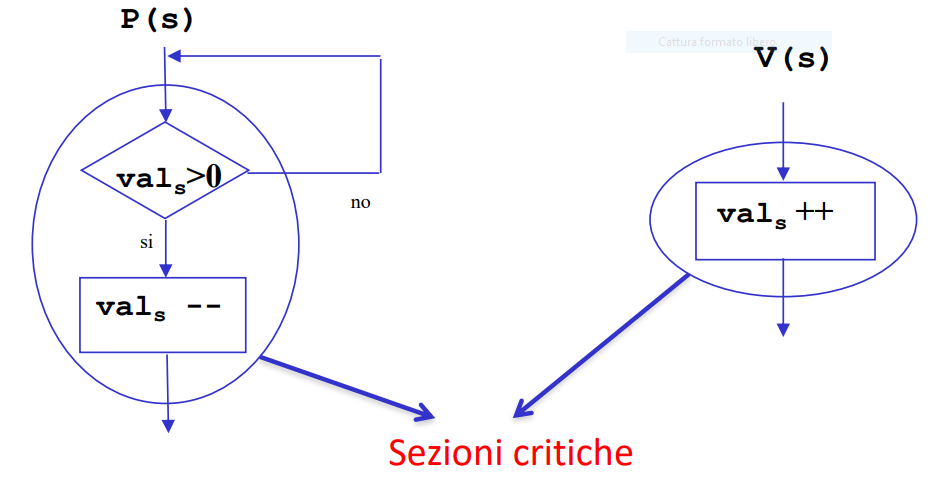
\includegraphics[width=0.50\columnwidth]{imgs/operazioni_semaforo.PNG}
\end{figure}

Quindi il semaforo viene utilizzato come strumento di sincronizzazione tra processi concorrenti:
\begin{itemize}
    \item \textbf{attesa}: P(s), val-s == 0
    \item \textbf{risveglio}: V(s), se vi è almeno un processo sospeso
\end{itemize}

\vspace{5mm}
\textbf{Proprietà del Semaforo}
\vspace{3mm}
Dato un semaforo S, siano:
\begin{itemize}
    \item \textbf{$val_s$}: valore dell'intero non negativo associato al semaforo;
    \item \textbf{$I_s$}: valore intero \>= 0 con cui il semaforo s viene inizializzato;
    \item \textbf{$nv_s$}: numero di volte che l'operazione V(s) è stata eseguita;
    \item \textbf{$np_s$}: numero di volte che l'operazione P(s) è stata completata.
\end{itemize}

\vspace{3mm}
Ad ogni istante possiamo esprimere il valore del semafor come:
\begin{center}
    $val_s = I_s + nv_s - np_s$
\end{center}

da cui ($val_s >= 0$):

\begin{center}
    \textbf{Relazione di Invarianza}

    \textbf{$np_s <= I_s + nv_s$}
\end{center}

La relazione di invarianza è sempre soddisfatta, per ogni semaforo, qualunque sia il suo valore e comunque sia strutturato il programma concorrente che lo usa.

\vspace{5mm}
Il semaforo è quindi uno strumento generale che consente la risoluzione di qualunque problema di sincronizzazione.

Esistono molti casi d'uso del meccanismo semaforico:
\begin{itemize}
    \item semafori di mutua esclusione
    \item semafori evento
    \item semafori binari composti
    \item semafori condizione
    \item semafori risorsa
    \item semafori privati
\end{itemize}

\vspace{5mm}
\textbf{Semaforo di mutua esclusione}

\vspace{3mm}
Il semaforo di mutua esclusione viene inizializzato ad 1. Principalmente viene utilizzato per realizzare le sezioni critiche di una stessa classe, secondo il protocollo:

\begin{lstlisting}
    class tipo_risorsa {
        <struttura dati di ogni istanza della classe>;

        semaphore mutex = 1;

        public void op1() {
            P(mutex);   // prologo
            <sezione critica: corpo della funzione op1>;
            V(mutex);   // epilogo
        }

        public void opN() {
            P(mutex);   // prologo
            <sezioen critica: corpo della funzione opN>;
            V(mutex);   // epilogo
        }
    }

    tipo_risorsa ris;
    ris.opi();
\end{lstlisting}

(il semaforo di mutua esclusione può assumere solo i valori 0 e 1)

\vspace{3mm}
In alcuni casi è consentito a più processi di eseguire contemporaneamente la stessa operazione su una risorsa, ma non operazioni diverse.

Quindi una soluzione protrebbe essere:
\begin{itemize}
    \item definisco un semaforo mutex per la mutua esclusione tra operazioni
    \item prologo ed epilogo di $op_i$ sono sezioni critiche quindi introduco un ulteriore semaforo di mutua esclusione $m_i$
\end{itemize}

Un esempio potrebbe essere il \textbf{problema dei lettori/scrittori}.

Sia data una risorsa condivisa F (ad esmepio un file) che può essere acceduta dai thread concorrenti in due modi:
\begin{itemize}
    \item \textbf{lettura};
    \item \textbf{scrittura}
\end{itemize}

\vspace{3mm}
Una possibile soluzione di sincronizzazione potrebbe essere:
\begin{itemize}
    \item la lettura è consentita a più thread contemporaneamente;
    \item la scrtittura è consentita ad un thread alla volta;
    \item lettura e scrittura su F non possono avvenire contemporaneamente
\end{itemize}

\begin{lstlisting}
    semaphore mutex = 1;
    semaphore ml = 1;
    int contl = 0;

    public void lettura(...) {
        P(ml);
        contl++;

        if(contl == 1) {
            P(mutex);
        }

        V(ml);
        <lettura del file>;
        P(ml);
        contl--;

        if(contl == 0) {
            V(mutex);
        }

        v(ml);
    }

    public void scrittura(...) {
        P(mutex);
        <scrittura del file>;
        V(mutex);
    }
\end{lstlisting}

\vspace{5mm}
\textbf{Semaforo evento}

\vspace{3mm}
Un semaforo evento è un semaforo binario utilizzato per imporre un \textbf{vincolo di precedenza} tra le operazioni dei processi. 
(ad es. $op_a$ deve essere eseguita da P1 solo dopo che P2 ha eseguito $op_b$).

\vspace{3mm}
Introduciamo quindi un semaforo \textbf{sem} inizializzato a \textbf{zero}:
\begin{itemize}
    \item prima di eseguire $op_a$, P1 esegue P(sem)
    \item dopo aver eseguito $op_b$, P2 esegue V(sem)
\end{itemize}

{
    problema del rendez-vous slide 48
}

\vspace{5mm}
\textbf{Semafori binari composti}

\vspace{3mm}
Un insieme di semafori usato in modo tale che:
\begin{itemize}
    \item uno solo di essi sia inizializzato a 1 e tutti gli altri a 0
    \item ogni processo che usa questi semafori esegue sempre sequenze che iniziano con la P su uno di questi e termina con la V su un altro.
\end{itemize}

Due processi P1 e P2 si scambiano dati di tipo T utilizzando una memoria condivisa (buffer).

Quindi devono esserci dei vincoli di sincronizzazione:
\begin{itemize}
    \item accessi al buffer mutuamente esclusivi
    \item P2 può prelevare un dato solo dopo che P1 lo abbia inserito
    \item P1, prima di inserire un dato, deve attendere che P2 abbia estratto il precedente
\end{itemize}

\begin{figure}[htbp]
    \centering
    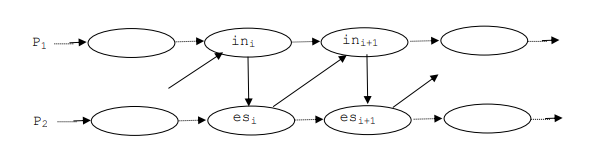
\includegraphics[width=0.60\columnwidth]{imgs/vincoli_precendenza.PNG}
\end{figure}

\vspace{3mm}
Utilizziamo quindi due semafori:
\begin{itemize}
    \item \textbf{vu}, per realizzare l'attesa di P1, in caso di buffer pieno
    \item \textbf{pn}, per realizzare l'attesa di P2, in caso di buffer vuoto
\end{itemize}

\vspace{3mm}
Buffer inizialmente vuoto, vu = 1, pn = 0
\vspace{3mm}

\noindent\begin{minipage}{.45\columnwidth}
    \begin{lstlisting}
        void invio(T dato) {
            P(vu);
            inserisci(dato);
            V(pn);
        }
    \end{lstlisting}
\end{minipage}\hfill
\begin{minipage}{.45\columnwidth}
    \begin{lstlisting}
        T ricezione() {
            T dato;
            P(pn);
            dato = estrai();
            V(vu);
            return dato;
        }
    \end{lstlisting}
\end{minipage}

\vspace{5mm}
\textbf{Semaforo condizione}

\vspace{3mm}
In alcuni casi l'esecuzione di un'istruzione S1 su una risorsa R è subordinata al verificarsi di una condizione C:

\begin{lstlisting}
    void op1(): region R << when(C) S1; >>
\end{lstlisting}

\vspace{3mm}
Il processo deve sospendersi se la condizione non è verificata e deve sucire dalla regione per consentire ad altri processi di eseguire altre operazioni su R
per rendere vera la condzione C.

\begin{figure}[htbp]
    \centering
    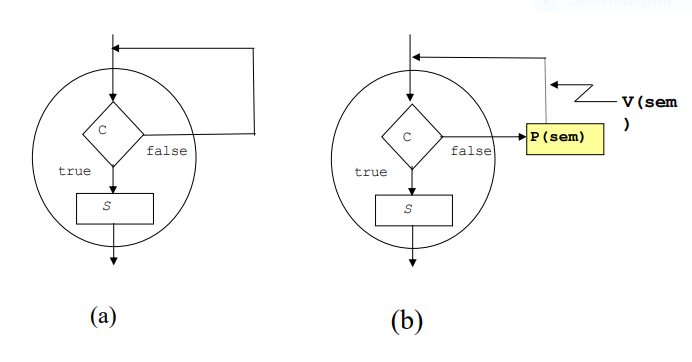
\includegraphics[width=0.70\columnwidth]{imgs/schema_condizione.PNG}
\end{figure}

\begin{itemize}
    \item Lo schema (a) presuppone una forma di attesa attiva da parte del processo che non trova soddisfatta la condizione
    \item Nello schema (b) si realizza la region sospendendo il processo sul semaforo sem da associare alla condizione.
    \begin{itemize}
        \item è necessaria un'altra operazione op2 che, chiamata da un'altro processo, modifichi lo stato interno di R in modo che C diventi vera
        \item nell'ambito di op2 viene eseguita la V(sem) per risvegliare il processo
    \end{itemize}
\end{itemize}

\vspace{3mm}
Schema con \textbf{attesa circolare}

\begin{lstlisting}
semaphore mutex = 1;
semaphore sem = 0;
int csem = 0;
\end{lstlisting}

\noindent\begin{minipage}{.45\columnwidth}
    \begin{lstlisting}
public void op1() {
    P(mutex);
    while(!C) {
        csem++;
        V(mutex);
        P(sem);
        P(mutex);
    }
    S1;
    V(mutex);
}
    \end{lstlisting}
\end{minipage}\hfill
\begin{minipage}{.45\columnwidth}
    \begin{lstlisting}
public void op2() {
    P(mutex);
    S2;
    if(csem > 0) {
        csem--;
        V(sem);
    }
    V(mutex);
}
    \end{lstlisting}
\end{minipage}

\vspace{3mm}
Schema con \textbf{passaggio di testimone}:

\begin{lstlisting}
semaphore mutex = 1;
semaphore sem = 0;
int csem = 0;
\end{lstlisting}

\noindent\begin{minipage}{.45\columnwidth}
    \begin{lstlisting}
public void op1() {
    P(mutex);
    if(!C) {
        csem++;
        V(mutex);
        P(sem);
        csem--;
    }
    S1;
    V(mutex);
}
    \end{lstlisting}
\end{minipage}\hfill
\begin{minipage}{.45\columnwidth}
    \begin{lstlisting}
public void op2() {
    P(mutex);
    S2;
    if(C && csem > 0) {
        V(sem);
    } else {
        V(mutex);
    }
}
    \end{lstlisting}
\end{minipage}

\vspace{3mm}
Questo secondo schema è più efficientre del primo ma ha comunque delle limitazioni. Permette di risvegliare un solo processo alla volta poichè ad uno solo può passare
il diritto di operare in mutua esclusione. Inoltre la condizione C (precondizione di S1) deve essere verificabile anche all'interno di op2. Ciò significa che
non deve contenere variabili locali o parametri della funzione op1.

\vspace{5mm}
\textbf{Semaforo condizione}

\vspace{3mm}
I semafori risorsa sono semafori generali, quindi possono assumere qualunque valore >= 0. Vengono generalmente impiegati per realizzare l'allocazione di risorse
equivalenti, nel quale il valore del semaforo rappresenta il numero di risorse libere.

\vspace{3mm}
\begin{lstlisting}
class tipo_gestore {
    semaphore mutex = 1;    // semaforo di mutua esclusione
    semaphore n_ris = N;    // semaforo risorsa
    boolean libera[N];      // indicatori di risorsa libera

    public tipo_gestore() {
        for(int i = 0; i < N; i++) {
            libera[i] = true;   // inizializzazione
        }
    }

    public int richiesta() {
        int i = 0;
        P(n_ris);
        P(mutex);
        while(libera[i] == false) {
            i++;
        }
        libera[i] = false;
        V(mutex);
        return i;
    }

    public ovid rilascio(int r) {
        P(mutex);
        libera[r] = true;
        V(mutex);
        V(n_ris);
    }
}
\end{lstlisting}

\vspace{3mm}
Leggere esempi sulle condizioni di sincronizzazione.

\vspace{5mm}
\textbf{Semaforo privato}

\vspace{3mm}
Un semaforo S si deive privato per un processo quando solo tale processo può eseguire la primitiva P sul semaforo S. La primitiva V sul semaforo può essere invece eseguita
da qualunque processo. Generalmente un semaforo privato viene inizalizzato con il valore zero.

\vspace{3mm}
I semafori privati vengono utilizzati per realizzare particolari politiche di allocazione di risorse:
\begin{itemize}
    \item il processo che acquisisce la risorsa può eventualmente sospendersi sul suo semaforo privato (se la condizione di sincronizzazione non è rispettata)
    \item chi rilascia la risorsa, risveglierà uno tra i processi sospesi, in base alla politica scelta, mediante una V sul semaforo privato del processo scelto.
\end{itemize}

\vspace{3mm}
Allocazione di risorse, \textbf{primo schema}:

\begin{lstlisting}
class tipo_gestore_risorsa {
    <struttura dati del gestore>;
    semaphore mutex = 1;
    semaphore priv[n] = {0, 0, ..., 0}; // semafori privati

    public void acquisizione(int i) {
        P(mmutex);
        if(<condizione di sincronizzazione>) {
            <allocazione della risorsa>;
            V(priv[i]);
        } else {
            <registra la sospensione del processo>;
        }
        V(mutex);
        P(priv(i));
    }

    public void rilascio() {
        int i;
        P(mutex);
        <rilascio della risorsa>;
        if(<esiste almeno un processo sospeso per il quale la condizione risulta true>) {
            <scelta fra i processi sospesi quello destinato alla riattivazione (Pi)>;
            <allocazione della risorsa a Pi>;
            <registrare che Pi non e piu sospeso>;
            V(priv[i]);
        }
        V(mutex);
    }
}
\end{lstlisting}

\vspace{3mm}
Proprietà del primo schema:
\begin{itemize}
    \item la sospensione del processo, nel caso in cui la condizione di sincronizzazione non sia soddisfatta, non può avvenire entro la sezione critica in quanto 
    ciò impedirebbe ad un processo che rilascia la risorsa di accedere a sua volta alla sezione critica e di riattivare il processo sospeso. E quindi la sospensione
    avviene fuori dalla sezione critica.
    \item la specifica del particolare algoritmo di assegnazione della risorsa non è opportuno che sia realizzata nella primitiva V.
    \item questo schema può presentare i seguanti problemi:
    \begin{itemize}
        \item l'operazione P sul semaforo privato viene sempre eseguita anche quando il processo richiedente non deve essere bloccato
        \item il codice relativo all'assegnazione della risorsa viene duplicato nelle procedure acquisizione e rilascio
    \end{itemize}
\end{itemize}

\vspace{3mm}
Allocazione di risorse, \textbf{secondo schema} (supera i limiti del primo):

\begin{lstlisting}
class tipo_gestore_risorsa {
    <struttura dati del gestore>;
    semaphore mutex = 1;
    semaphore priv[n] = {0, 0, ..., 0};

    public void acquisizione(int i) {
        P(mutex);
        if(! <condizione di sincronizzazione>) {
            <registrare la sospensione del processo>;
            V(mutex);
            P(priv[i]);
            <resitrare che il processo non e piu sospeso>;
        }
        <allocazione della risorsa>;
        V(mutex);
    }

    public void rilascio() {
        int i;
        P(mutex);
        <rilascio della risorsa>;
        if(<esiste almeno un processo sospeso per il quale la condizione risulta true>) {
            <scelta del processo Pi da riattivare>;
            V(priv[i]);
        } else {
            V(mutex);
        }
    }
}
\end{lstlisting}

\vspace{3mm}
Rispetto al primo schema, in questa soluzione risulta più complesso realizzare la riattivazione di più processi per i quali risulti vera contemporaneamente la
condizione di sincronizzazione. Infatti il processo che rilascia la risorsa attiva al più un processo sospeso, il quale dovrà a sua volta provvedere alla riattivazione
di eventuali altri processi.

\section{Realizzazione del nucleo}

Si chiama \textbf{nucleo} (o kernel) il modulo (o insieme di funzioni) realizzato in software, hardware o firmware che supporta il concetto di processo e realizza
gli strumenti necessari per la gestione dei processi.

\vspace{3mm}
Il nucleo costituisce il livello più interno di un qualunque sistema basato su processi, ad esempio:
\begin{itemize}
    \item il livello più elementare di un sistema operativo multiprogrammato
    \item il supporto a tempo di esecuzione di un linguaggio per la programmazione concorrente
\end{itemize}

Il nucleo è il solo modulo che è consio dell'esistenza delle interruzioni. I processi che colloquiano con i dispositivi utilizzano opportune primitive del
nucleo che provvedono a sospenderli in attesa del completamento dell'azione richiesta. Non appena l'azione viene completata, il relativo segnale di interruzione
iviato dal dispositivo alla CPU viene catturato dal nucleo che provvede a risvegliare il processo sospeso.

La gestione delle interruzioni è quindi invisibile ai processi ed ha come unico effetto rilevabile di rallentare la loro esecuzione sulle rispettive macchine virtuali.

\subsection{Caratteristiche fondamentali del nucleo}

\textbf{Efficienza}: condiziona l'intera struttura a processi. Infatti esistono dei sistemi in cui alcune o tutte le operazioni del nucleo sono realizzate in hardware
o attraverso microprogrammi.

\vspace{3mm}
\textbf{Dimensioni}: la semplicità delle funzioni richieste al nucleo fa si che la sua dimensinoe risulti estremamente limitata.

\vspace{3mm}
\textbf{Separazioen tra meccanismi e politiche}: il nucleo deve contenere solo meccanismi consentendo così, a livello di processi, di utilizzare tali meccanismi per la 
realizzazione di diverse politiche di gestione a seconda del tipo di applicazione.

\begin{figure}[htbp]
    \centering
    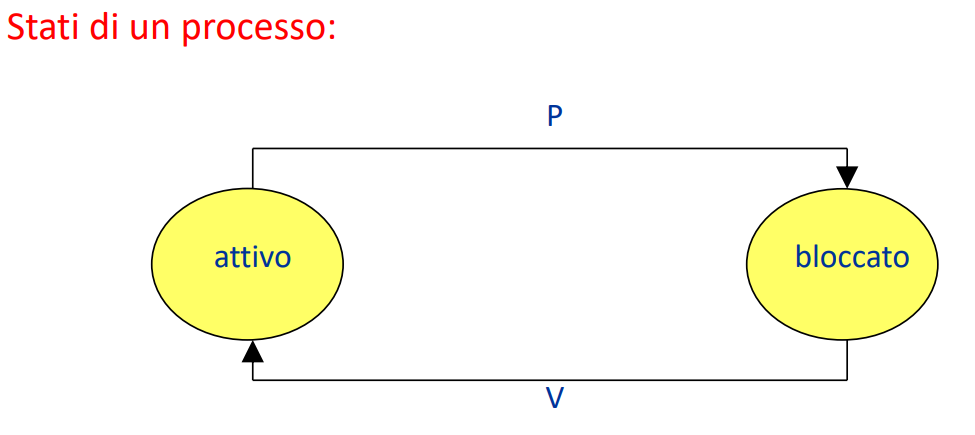
\includegraphics[width=0.70\columnwidth]{imgs/processo.PNG}
\end{figure}

Le transizioni tra i due stati sono implementate dai meccanismi di sincronizzazione realizzati dal nucleo. \textbf{P} per sospensione e \textbf{V} per risveglio.

\vspace{3mm}
Stati di un processo in un sistema in cui il numero di processi supera il numero delle unità di elaborazione:
\begin{figure}[htbp]
    \centering
    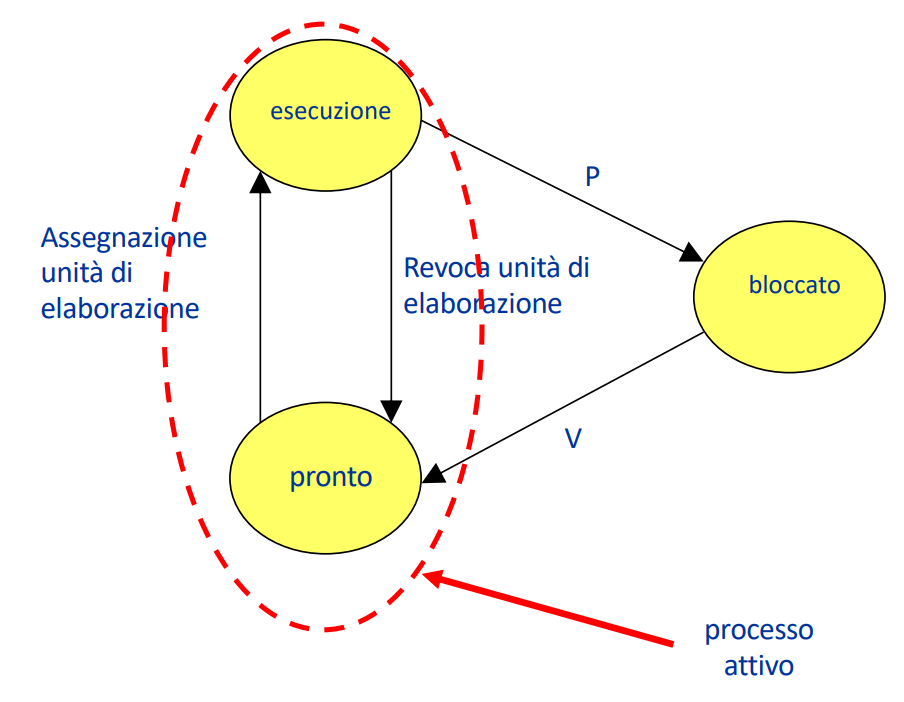
\includegraphics[width=0.70\columnwidth]{imgs/processi.PNG}
\end{figure}

Quando un processo perde il controllo del processore, il contenuto dei registri del processo viene salvato in un'area di memoria associata al processo, chiamata descrittore.

Ciò consente una maggiore flessibilità nella politica di assegnazione del processore ai processi, rispetto alla soluzione di salvare le informazioni nello stack.

\vspace{3mm}
Quindi la funzione fondamentale del nucleo di un sistema a processi è la gestione delle transizioni di stato dei processi. I principali compiti del nucleo sono:
\begin{itemize}
    \item \textbf{Gestire il salvataggio e il ripristino dei contesti dei processi}: quando un processo abbandona il controllo dell'unità di elaborazione fisica,
        tutte le informazioni contenute nei registri di tale unità devono essere trasferite nel descrittore. Allo stesso modo, quando un processo riprende l'esecuzione
        tutte le informazioni contenute nel suo descrittore devono essere trasferite nei registri di macchina
    \item \textbf{Scegliere a quale tra i processi pronti assegnare l'unità di elaborazione (scheduling della CPU)}: quando un processo abbandona il controllo
        dell'unità di elaborazione, il nucleo deve scegliere tra tutti i processi pronti quello da mettere in esecuzione. La scelta può essere o di tipo FIFO, oppure
        può utilizzare la priorità dei processi.
    \item \textbf{Gestire le interruzioni dei dispositivi esterni}: traducendole in attivazione di processi da bloccato a pronto.
    \item \textbf{Realizzare i meccanismi di sincronizzazione dei processi}: gestendo il passaggio dei processi dallo stato di esecuzioen allo stato di bloccato e da
        bloccato a pronto.
\end{itemize}

\subsection{Realizzazione del Nucleo: Architettura monoprocessore}

\subsubsection{Strutture Dati del Nucleo}






\section{Modello a scambio di messaggi}







\end{document}
